\chapter{Results}
In this chapter, the obtained results from the defined experiments in section \ref{sec:experiments} are presented. In section \ref{sec:exp_feas} we summarized the results for the feasibility test of a deep-learning based peripheral nerve segmentation.
Section \ref{sec:exp_3dcontext} presents the achieved performances for the defined segmentation metrics for the different neural network architectures with variable access to 3D information.
In section \ref{sec:exp_pp} the results for the impact-study of post-processing applied to the segmentation of the baseline architecture and the best performing 3D architecture, respectively.
Finally, section \ref{sec:exp_evaluation} features the results obtained concerning the inter-rater variability, to which we compare and evaluate our best performing 3D architecture.
The detailed results of the individual experiments can be found in the appendix \ref{app:results}.
\section{Experiment 1: Feasibility} \label{sec:exp_feas}

\begin{figure}[htbp]
	\centering
	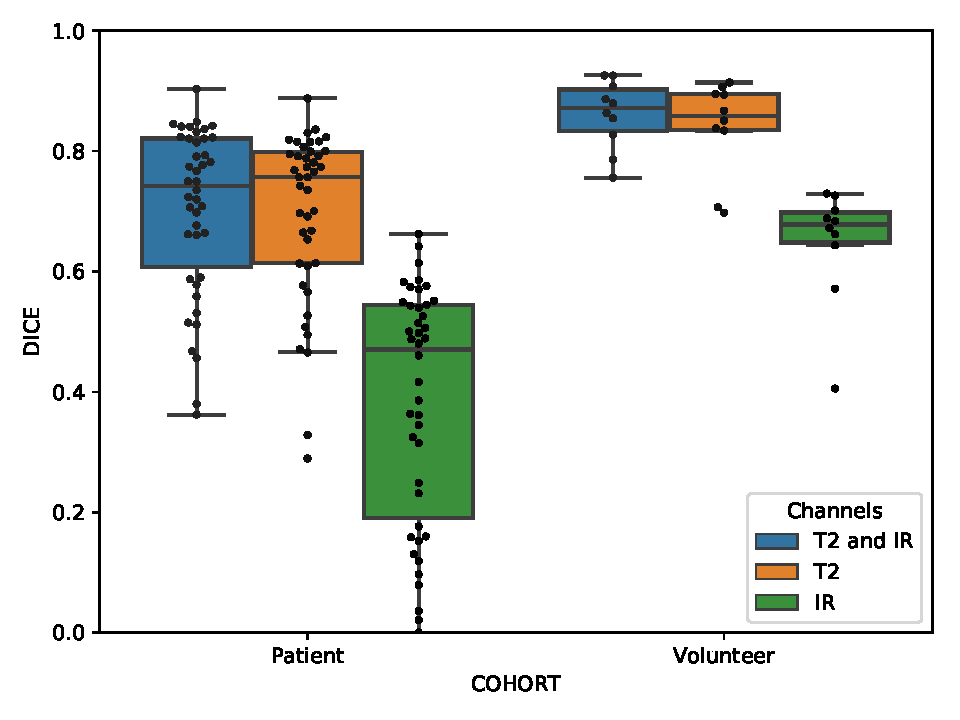
\includegraphics[width=0.8\textwidth]{boxplot_T2_IR_DICE}
    \caption[Boxplot for the \acrlong{dice} for the Baseline trained on T2 and IR separately.]{Boxplot for the \acrlong{dice} for the baseline architecture trained on both, T2 and IR, images as well as trained on each image channel separately. Note that comparable segmentation performance is achieved by only incorporating the T2 image channel. Using only the IR channel, however, results in a significant performance drop.}
    \label{fig:results_boxplot_T2_IR_dice}
\end{figure}




\section{Experiment 2: 3D Context} \label{sec:exp_3dcontext}
\section{Experiment 3: Post-processing} \label{sec:exp_pp}
\section{Evaluation} \label{sec:exp_evaluation}
\endinput